\newpage
\section{Example 1: Closed-set identification of words in noise with
figures}

\subsection{General description of the experiment} See
\filename{examples/manual/closedsetword.apx}. This is an example
of a closed-set identification test for children. A word (wave
file) is presented and the child responds by clicking on one of
four figures on the screen(figure~\ref{fig:closedset}).
Subsequently, a new set of figures is shown, and again, a word
corresponding to one of these figures is routed to the sound card.
This is repeated 3 times. The three words are embedded in noise at
a certain signal-to-noise ratio. In this example the level of the
noise is fixed and the level of the word varies. At the beginning
of the experiment \apex queries for the SNR (signal to noise
ratio, in dB). After having entered this value four figures will
appear. Press Start to start the experiment and to hear the first
stimulus (speech in noise). After the experiment has finished the
results are written to a results file and the percentage correct
is determined.

\index{Example: closed-set identification}

\begin{figure}
 \centering
%% 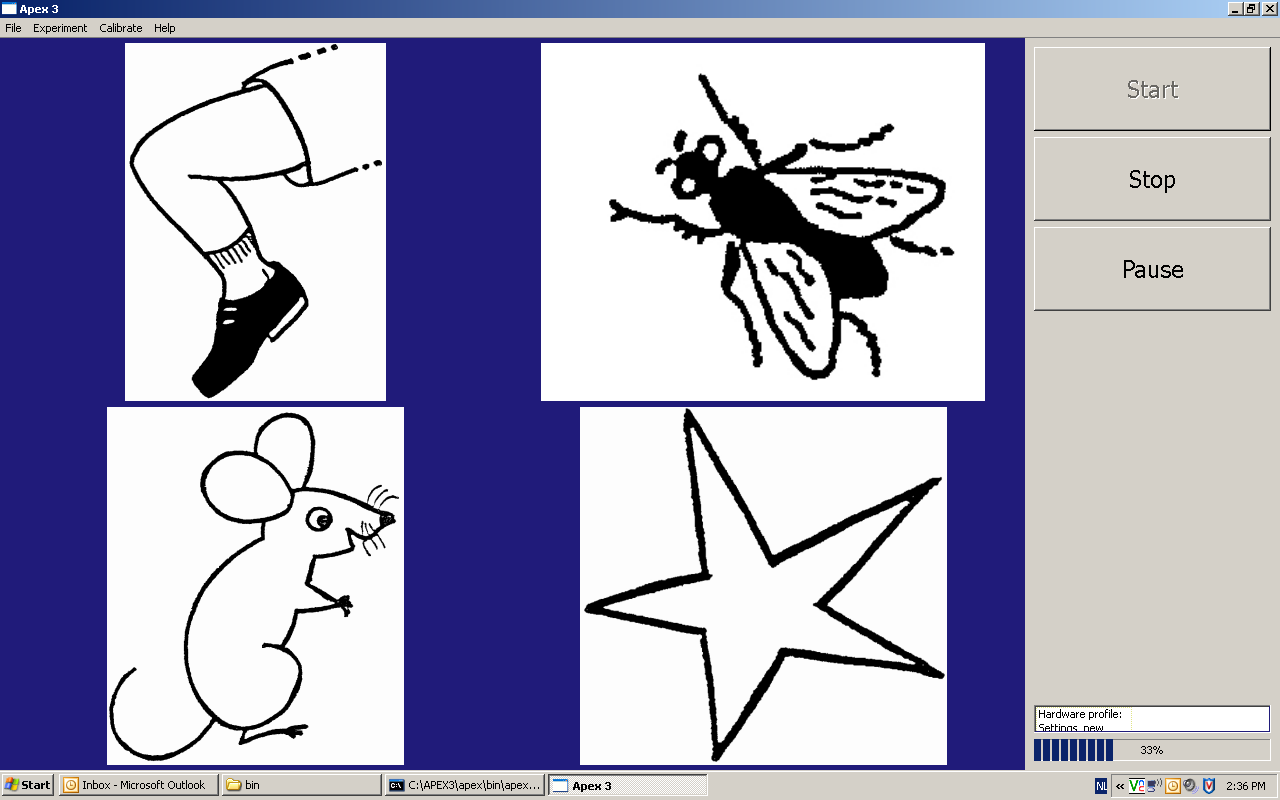
\includegraphics[width=\textwidth]{example1closedset.png}
 \caption{Example of closed-set identification experiment}
 \label{fig:closedset}
\end{figure}

\subsection{Conceptual}
The experiment as described in the previous paragraph should first
be translated to concepts understood by \apex. The main concepts
in this example are \textbf{datablock}, \textbf{stimulus},
\textbf{screen} and \textbf{procedure}. For each of the 3 words to
be presented to the subject, a wave file is available on disk. For
each wave file, a datablock is defined, and for each resulting
datablock a stimulus is defined. Everything that is defined is
assigned an ID, to be able to refer to it later on. Therefore, now
we have 3 stimuli with IDs \id{stimulus_star}, \id{stimulus_mouse}
and \id{stimulus_fly}.

We should also define the things to be shown on the screen during
the experiment. This is done by defining a screen for each word.
Each screen contains 4 pictures, of which one corresponds to the
word. Each screen again gets an ID, in this case we name the
screen by the pictures it contains. Therefore we now have 3
screens with ID \id{screenstar_horse_vase_moon},
\id{screenknee_fly_mouse_star} and \id{screenmouse_fly_star_moon}.

To indicate the order in which the words should be presented, and
together with which screen, a procedure is defined. In the
procedure a number of trials is defined. Recall that a trial is
the combination of a screen, a stimulus and a correct answer.
Therefore a trial is a way to link each of our stimuli with a
screen.

Now only the output logic remains to be defined. The idea is to
continuously present a noise signal and to set the level of the
words such that a certain SNR is obtained. To achieve this, we
define 2 filters, the first one is a generator (i.e., a filter
without input channels) that will generate the noise signal. The
other one is an amplifier, which will amplify or attenuate the
words to obtain the desired SNR.

In the following sections each of the elements of the \xml{XML}
file necessary to implement the latter concepts will be described
in detail. The first one is \element {procedure}.

\subsection{Detailed description of various elements}
\begin{lstlisting}
  <procedure xsi:type="apex:constantProcedure">
    <parameters>
      <presentations>1</presentations>
      <order>sequential</order>
    </parameters>
    <trials>
      <trial id="trial_star">
        <answer>picturestar</answer>
        <screen id="screenstar_horse_vase_moon"/>
        <stimulus id="stimulus_star"/>
      </trial>
      <trial id="trial_fly">
        <answer>picturefly</answer>
        <screen id="screenknee_fly_mouse_star"/>
        <stimulus id="stimulus_fly"/>
      </trial>
      <trial id="trial_mouse">
        <answer>picturemouse</answer>
        <screen id="screenmouse_fly_star_moon"/>
        <stimulus id="stimulus_mouse"/>
      </trial>
    </trials>
  </procedure>
\end{lstlisting}

The attribute \xml{xsi:type="apex:constantProcedureType"}
indicates that a constant stimuli procedure is used. This means
that the procedure will select the next trial from the trial list
and that it completes after every trial has been presented a
certain number of times.
\begin{itemize}

\item \element{parameters} defines the behavior of the procedure
\begin{itemize}

\item \element{presentations} every trial is presented once

\item \element{order} \xml{sequential} the three trials are
presented sequentially, in the order that is specified in the
experiment file
\end{itemize}
\index{presentations} \index{order}

\item \element{trials} contains different \element{trial} elements
to specify a trial. After selecting a trial the
\element{procedure} will show the specified screen and send the
stimulus to the device. Each trial is given an ID (arbitrary
name), eg \id{TrialStar}, such that it can be referred to later on
or viewed in the results file.

\item \element{answer} the correct answer, to be used by \apex to
determine whether the subject's response is correct. Here, the
subject gets the opportunity to click on one of 4 pictures. The
result from the screen (the subject's response) will be the ID of
the element of the screen that was clicked. Therefore, in this
example, we specify the ID of the picture corresponding to the
stimulus that is presented.
\end{itemize}

A trial must be defined for all the words of the experiment.

\index{trial} \index{answer} \index{screen} \index{stimulus}

\begin{lstlisting}
    <corrector xsi:type="apex:isequal"/>
\end{lstlisting}
\index{corrector}

The corrector checks whether the response is correct or not. The
attribute \xml{xsi:type="apex:isequal"} compares whether the two
input values are exactly the same. In this example
\element{corrector} compares the answer specified under trial and
the ID corresponding to the picture that has been clicked.

\begin{lstlisting}
<screens>
    <uri_prefix>closedset</uri_prefix>
    <reinforcement>
      <progressbar>true</progressbar>
      <feedback length="600">false</feedback>
    </reinforcement>
    <screen id="screenstar_horse_vase_moon">
      <gridLayout height="2" width="2">
        <picture id="picturestar" row="1" col="1">
          <path>star.jpg</path>
        </picture>
        <picture id="picturehorse" row="2" col="1">
          <path>horse.jpg</path>
        </picture>
        <picture id="picturevase" row="1" col="2">
          <path>vase.jpg</path>
        </picture>
        <picture id="picturemoon" row="2" col="2">
          <path>moon.jpg</path>
        </picture>
            </gridLayout>
      <buttongroup id="buttongroup1">
        <button id="picturestar"/>
        <button id="picturehorse"/>
        <button id="picturevase"/>
        <button id="picturemoon"/>
      </buttongroup>
      <default_answer_element>buttongroup1</default_answer_element>
    </screen>
    <screen id="screenknee_fly_mouse_star">
      <gridLayout height="2" width="2">
        <picture id="pictureknee" row="1" col="1">
          <path>knee.jpg</path>
        </picture>
        <picture id="picturefly" row="2" col="1">
          <path>fly.jpg</path>
        </picture>
        <picture id="picturemouse" row="1" col="2">
          <path>mouse.jpg</path>
        </picture>
        <picture id="picturestar" row="2" col="2">
          <path>star.jpg</path>
        </picture>
      </gridLayout>
      <buttongroup id="buttongroup2">
        <button id="pictureknee"/>
        <button id="picturefly"/>
        <button id="picturemouse"/>
        <button id="picturestar"/>
      </buttongroup>
      <default_answer_element>buttongroup2</default_answer_element>
    </screen>
    <screen id="screenmouse_fly_star_moon">
      <gridLayout height="2" width="2">
        <picture id="picturemouse" row="1" col="1">
          <path>mouse.jpg</path>
        </picture>
        <picture id="picturefly" row="2" col="1">
          <path>fly.jpg</path>
        </picture>
        <picture id="picturestar" row="1" col="2">
          <path>star.jpg</path>
        </picture>
        <picture id="picturemoon" row="2" col="2">
          <path>moon.jpg</path>
        </picture>
      </gridLayout>
      <buttongroup id="buttongroup3">
        <button id="picturemouse"/>
        <button id="picturefly"/>
        <button id="picturestar"/>
        <button id="picturemoon"/>
      </buttongroup>
      <default_answer_element>buttongroup3</default_answer_element>
    </screen>
  </screens>
\end{lstlisting}

\element{screens} contains several \element{screen} elements that
can be referred to elsewhere in the experiment file (e.g., in
\element{procedure} above).

\begin{itemize}
\item \element{uri_prefix} a relative path is specified here
(relative with respect to the experiment file). Since \apex knows
the location of the experiment file, only the folder containing
the wave files and pictures must be specified. It is also possible
to give the absolute path, starting at the root. There are 3 ways
to specify a prefix: by directly specifying an absolute path, by
directly specifying a path relative to the experiment file or by
referring to a prefix stored in \filename{apexconfig.xml}. Please
refer to section~\ref{sec:prefixes} for more information.

\item \element{reinforcement} includes

\begin{itemize}

\item \element{progressbar} As the value is \xml{true} a
progressbar will be displayed in the right hand bottom corner of
the screen that indicates how many trials have been completed and
how many remain.

\item \element{feedback length} duration of time after response
(in msec) that \apex waits before presenting the next trial.
During this interval, feedback can be displayed. In this case, no
feedback (thumb up, thumb down) is given as the value is
\xml{false}.

\end{itemize}
\end{itemize}

\begin{itemize}
\item \element{screen} For each word to be presented, a screen is
defined. Each screen has an ID by which it can be referred to
elsewhere in the experiment file (e.g. in \element{trials} to
associate it with a stimulus).
\begin{itemize}

\item \element{gridLayout} specifies how the four figures will be
arranged on the screen. A GridLayout creates a regular grid on the
screen with the specified number of rows and columns. In this
example there are 2 rows and 2 columns. Each figure is defined by
means of a \element{picture} element. Such a definition can be
seen as associating a graphics file with an ID and specifying at
what position of the layout it should be shown. In this case, jpeg
files are used, but other formats are also possible (e.g., png,
bmp, gif).

\begin{itemize}
\item \element{picture}


\element{uri} since the prefix as specified under
\element{uri_prefix} is preprended to each \element {uri}  it
suffices to give the name of the .jpeg file in \element{path}. The
path is relative to the experiment file.

\end{itemize}
\end{itemize}
\begin{itemize}
\item \element{buttongroup} defines a group of screen elements,
namely those (four figures) that are displayed on the screen. The
ID is defined before.

\item \element{default_answer_element} As many elements can be
defined in a screen, \apex has no way to know which element
contains the subject's response. If, for example, a text box is
shown and 2 buttons, it is unclear which is to be used to
determine whether the answer is correct or not. Therefore, in
\element{default_answer_element} the element is designated that
contains the subject's response. In the case of screen elements
that are clicked in order to respond, the example is further
complicated by the fact that we cannot specify just one of the
elements (buttons, pictures), but the response rather comes from a
group of elements. This is when a \element{buttongroup} can be
used to group together different screen elements.
\end{itemize}
\end{itemize}
\index{screens} \index{uri prefix} \index{reinforcement}
\index{progressbar} \index{feedback length} \index{screen}
\index{gridlayout} \index{picture} \index{path}
\index{buttongroup} \index{default answer element}

In this example 5 datablocks are defined, 3 for the word files, 1
for the noise and 1 for silence.

\begin{lstlisting}
 <datablocks>
    <uri_prefix>closedset/</uri_prefix>
    <datablock id="datablock_star">
      <device>wavdevice</device>
      <uri>star.wav</uri>
    </datablock>
    <datablock id="datablock_fly">
      <device>wavdevice</device>
      <uri>fly.wav</uri>
    </datablock>
    <datablock id="datablock_mouse">
      <device>wavdevice</device>
      <uri>mouse.wav</uri>
    </datablock>
    <datablock id="noisedata">
      <device>wavdevice</device>
      <uri>noise.wav</uri>
    </datablock>
    <datablock id="silence">
      <device>wavdevice</device>
      <uri>silence:500</uri>
    </datablock>
  </datablocks>
\end{lstlisting}
\index{datablocks}

\element{datablocks} contains 5 \element{datablock} elements and a
prefix.
\begin{itemize}
\item \element{uri_prefix} a relative path is specified here. It
is also possible to give the absolute path, starting at the root
(see section~\ref{sec:prefixes}).

\item \element{datablock} For each wave file a datablock is made,
with an ID.  \item Each datablock is associated to a
\element{device} (by means of the ID of the device). In datablock
\id{silence} the special syntax is demonstrated for creating a
datablock containing only silence (i.e., all samples are zeros).
This is done to prevent the speech and noise from starting at the
same time. The length of the silence datablock is specified in ms
after the prefix \xml{silence}. It is added before the signal, not
before the noise.

\end{itemize}
\index{datablocks} \index{uri prefix} \index{datablock}
\index{device} \index{uri}

A datablock must be made for all wave files used in the
experiment, including the noise (that will be used by the noise
generator).



In the next sections, the output logic will be defined.
Figure~\ref{fig:ex1-output} gives an overview of the building
blocks that are used in this example. On the left hand side the
datablocks are shown. In the middle the noise generator and the
amplifier and on the right hand side the sound card. As the words
are to be amplified or attenuated according to the desired SNR,
the corresponding datablocks are routed through the amplifier.

\begin{figure}
 \centering
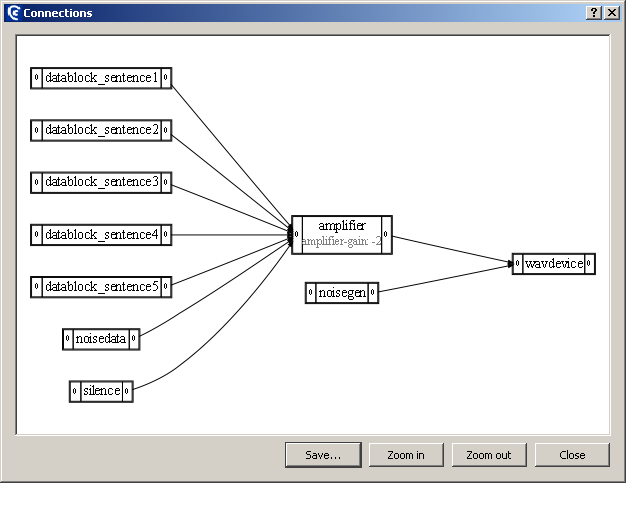
\includegraphics[width=0.5\textwidth]{connectionswindow.png}
 \caption{The connection window}
 \label{fig:ex1-output}
\end{figure}

In the next element the output device is specified.

\begin{lstlisting}
 <devices>
    <device id="wavdevice" xsi:type="apex:wavDeviceType">
      <driver>portaudio</driver>
      <card>default</card>
      <channels>1</channels>
      <samplerate>44100</samplerate>
    </device>
  </devices>
\end{lstlisting}
\index{devices}

All devices defined in the experiment file are grouped in
\element{devices}. In this example there is only 1
\element{device} element. Its ID is set to \id{soundcard}. As an
ID is unique for an entire experiment file, it can be used later
on to refer to this device.

\begin{itemize}
\item  The \xml{xsi:type="apex:wavDeviceType"} attribute tells
\apex that a sound card is used. The experiment only starts if all
devices can be opened.

\item \element{driver} specifies the software driver to be used
for sound output. If unsure, set it to \xml{portaudio}.

\item \element{card} specifies the name of the sound card to be
used. The system default card can be used by specifying
\xml{default} as a card name. Other card names can be defined in
\filename{apexconfig}.

\item \element{channels} specifies the number of channels of the
sound card to be used. The number of channels is restricted to the
selected sound card, with a maximum of 2 for portaudio.

\item \element{samplerate} the sampling rate of the sound card;
Not all sampling rates are supported by all devices, and some
drivers automatically convert the sampling rate. Check your sound
card documentation. The sample rate of the sound card should
correspond to the sampling rates of all datablocks used with it.
If not, an error message will be shown.

\end{itemize}

\index{device} \index{driver} \index{card} \index{channels}
\index{gain} \index{samplerate}

Filters must be defined whenever the signal (or noise) is
manipulated. In this example the level of the noise remains
constant and the signal is amplified or attenuated using an
amplifier filter (loop of \element{datablock}).

\begin{lstlisting}
<filters>
    <filter xsi:type="apex:dataloop" id="noisegen"> (*@\label{xml:filter1}@*)
      <device>wavdevice</device>
      <channels>1</channels>
      <continuous>false</continuous>
      <datablock>noisedata</datablock>
      <basegain>-5</basegain>
      <gain id="noisegain">0</gain>
      <randomjump>true</randomjump>
    </filter>
    <filter xsi:type="apex:amplifier" id="amplifier">  (*@\label{xml:filter2}@*)
      <device>wavdevice</device>
      <channels>1</channels>
      <basegain>-5</basegain>
      <gain id="gain">0</gain>
    </filter>
  </filters>
\end{lstlisting}
\index{filter}

\element{filters} contains individual \element{filter} elements,
which specify a filter, or as a special case a generator (i.e., a
filter without input channels).
\begin{itemize}

\item \element{filter} on line~\ref{xml:filter1} the attribute
\xml{xsi:type="apex:dataloop"} tells \apex that a dataloop
generator has to be created. This is a generator that takes a
datablock and loops it infinitely. The datablock to be looped is
specified by its ID \id{noisedata}. The dataloop generator itself
is assigned the ID \id{noisegen}.


\item \element{filter} on line~\ref{xml:filter2} the attribute
\xml{xsi:type="apex:amplifier"} tells \apex that an amplifier is
to be created. The gain of this amplifier will be varied to change
the amplitude of the words and thus the SNR. It is assigned ID
\id{amplifier}. The gain of the amplifier is made a variable
parameter by assigning it ID \id{gain}
\begin{itemize}
\item \element{device} The device with which the filter is
associated \item \element{channels} The number of channels of the
filter. The available number of channels is dependent on the type
of filter. An amplifier can have any number of channels.

\item If \element{continuous} is set to \xml{true}, the filter or generator
will keep on running in between two trials (i.e., when the subject is responding).
 In this example it stops when the stimulus stops playing (\xml{false}).

\item \element{datablock} The datablock with ID noisedata,
specified under \element{datablocks} will be looped.

\item \element{basegain} the total gain of the amplifier is
basegain+gain. Basegain cannot be a parameter, gain can be a
parameter. The total gain of the complete output system should not
be larger than 0 to avoid clipping of the signal. This is why
basegain = -5.

\item \element{gain} extent to which the signal is amplified.

\item If \element{randomjump} is set to \xml{true}, when the dataloop is started, it will jump to a random sample in the datablock. Thereafter it is looped.
\end{itemize}
\end{itemize}

\index{filters} \index{filter} \index{device} \index{channels}
\index{continuous} \index{datablock} \index{basegain} \index{gain}
\index{randomjump}

\begin{lstlisting}
<stimuli>
    <stimulus id="stimulus_star">
      <datablocks>
        <sequential>
          <datablock id="silence"/>
          <datablock id="datablock_star"/>
          <datablock id="silence"/>
        </sequential>
      </datablocks>
    </stimulus>
    <stimulus id="stimulus_fly">
      <datablocks>
        <sequential>
          <datablock id="silence"/>
          <datablock id="datablock_fly"/>
          <datablock id="silence"/>
        </sequential>
      </datablocks>
    </stimulus>
    <stimulus id="stimulus_mouse">
      <datablocks>
        <sequential>
          <datablock id="silence"/>
          <datablock id="datablock_mouse"/>
          <datablock id="silence"/>
        </sequential>
      </datablocks>
    </stimulus>
  </stimuli>
\end{lstlisting}
\index{stimuli} \index{datablocks}


\element{stimuli} contains different \element{stimulus}, each with
an ID \element{stimulus}

\begin{itemize}\item \element{datablocks}
can be combined in \element{sequential} order (as opposed to
\element{simultaneous}.
\end{itemize}

This is repeated for all the stimuli in the experiment.

\index{stimuli} \index{stimulus} \index{datablocks}
\index{sequential}

\begin{lstlisting}
<connections>
    <connection>
      <from>
        <id>_ALL_</id>
        <channel>0</channel>
      </from>
      <to>
        <id>amplifier</id>
        <channel>0</channel>
      </to>
    </connection>
    <connection>                (*@\label{xml:cha}@*)
      <from>
        <id>amplifier</id>
        <channel>0</channel>
      </from>
      <to>
        <id>wavdevice</id>
        <channel>0</channel>
      </to>
    </connection>               (*@\label{xml:chb}@*)
    <connection>                (*@\label{xml:chc}@*)
      <from>
        <id>noisegen</id>
        <channel>0</channel>
      </from>
      <to>
        <id>wavdevice</id>
        <channel>0</channel>
      </to>
    </connection>               (*@\label{xml:chd}@*)
  </connections>

\end{lstlisting}
\index{connections}

\index{channel}

\element{connections} defines how the different datablocks and
filters are routed to the output device. The ID \id{_ALL_} stands
for all the datablocks. In this example they are routed to the
first channel of the filter with ID {amplifier} (defined under
\element{filters}). In the amplifier the signal is amplified or
attenuated and sent to the wavdevice on lines~\ref{xml:cha}
to~\ref{xml:chb}. At the same time the noise, generated by a
generator with ID noisegen, is sent to the same channel of the
wavdevice. The channels are numbered from 0 onwards. The level of
the noise remains constant and does not pass through an amplifier
(lines~\ref{xml:chc} to~\ref{xml:chd}).

A visual representation of connections can be obtained by choosing
``Show stimulus connections'' under ``Experiment''in the main
\apex menu (top left menu bar).

\todo{idn1 xslt is outdated, we now use javascript results}

\begin{lstlisting}
<results>
   <xsltscript>idn.xsl</xsltscript>
</results>
\end{lstlisting}

Even if \element{results} is not specified in the experiment file
\apex will deliver a results file in XML.
\begin{itemize}
\item \element{xsltscript}  a script can transform the XML data to
an easier readable format; this script can be stored in folder
\filename{scripts} under \apex. For more information please read
section~\ref{sec:Using XSLT transforms}.
\end{itemize}
\index{results} \index{xsltscript}

\begin{lstlisting}
<interactive>
   <entry type="int" description="SNR in dB"
    expression="/apex:apex/filters/filter[@id='amplifier']/gain"
    default="0"/>
 </interactive>
\end{lstlisting}

If a small part of an experiment file has to be changed right
before the start of an experiment (e.g. a start value, a gain
value, the subject's name), \apex can show the experimenter a
small \ac{gui} containing the elements to be changed. This is
accomplished by defining the \element{interactive} element in the
experiment file.

In this example we will modify the gain of the filter with ID
\id{amplifier} to a value that is entered by the experimenter at
the start of the experiment.

It is only possible to change the value of an existing element of the experiment file, elements cannot be added. For each element to be changed, an \element{entry} should be defined under \element{interactive}. \element{entry} has  four attributes that should be defined:

\begin{itemize}
\item \attribute{type} specifies the type of input element that
will be shown. If it is \xml{int}, a spinbox\footnote{A spinbox is
an input field that only accepts numbers and has 2 buttons to
respectively increase or decrease its value} will be shown. If it
is \xml{string} a plain text box will be shown. In this case a
spinbox will be shown as a gain is always numeric. \item
\attribute{description} defines the text to be shown in the
\ac{gui} next to the input element, such that the experimenter
knows exactly what to fill in. \item \attribute{expression}
defines the element of the experiment file to be changed. It is
specified by a so-called XPath expression \footnote{see
\url{http://www.w3.org/TR/xpath}}. For a description of XPath, we
refer to the according standard or a good XML book.

\oxygen{OxygenXML can generate XPath expressions for you. First
point the cursor to the target element, then click the right mouse
button and select. An XPath expression to the clicked location is
now in the clipboard and can be pasted at the appropriate place
using the paste function.} \item \attribute{default} specifies the
default value to be shown in the input element.
\end{itemize}

\index{interactive} \index{entry type} \index{expression}

\todo{the elements below are now under the <results> tag}

\begin{lstlisting}
<general>
    <showresults>true</showresults>
    <saveprocessedresults>true</saveprocessedresults>
</general>
\end{lstlisting}

\element{general} defines some general parameters. Saving
processed results in a results file is only possible if a
XSLT-script is defined. See section~\ref{sec:Using XSLT
transforms}.

\begin{itemize}
\item \element{showresults} If \xml {true} a window will appear
after completion of the experiment asking whether the results
should be shown on screen.

\item \element{saveprocessedresults} If \xml {true} the
experimenter will be asked whether the processed results must be
appended to the results file.
\end{itemize}

\index{general} \index{showresults} \index{saveprocessedresults}
